% This is samplepaper.tex, a sample chapter demonstrating the
% LLNCS macro package for Springer Computer Science proceedings;
% Version 2.20 of 2017/10/04
%
\documentclass[runningheads]{llncs}
%
\usepackage{graphicx}
\usepackage{amsmath}
% Used for displaying a sample figure. If possible, figure files should
% be included in EPS format.
%
% If you use the hyperref package, please uncomment the following line
% to display URLs in blue roman font according to Springer's eBook style:
% \renewcommand\UrlFont{\color{blue}\rmfamily}

\begin{document}
%
\title{Early-stage nodule generation with deep image prior}
%
%\titlerunning{Abbreviated paper title}
% If the paper title is too long for the running head, you can set
% an abbreviated paper title here
%
\author{Octavio E. Martinez Manzanera\inst{1} \and
Vasileios Baltatzis\inst{1} \and
Sujal Desai\inst{2,3} \and
Anand Devaraj\inst{2} \and
Sam Ellis\inst{1} \and
Loic Le Folgoc\inst{3} \and
Arjun Nair\inst{4} \and
Ben Glocker\inst{3} \and
Julia Schnabel\inst{1}}
%
\authorrunning{O.E. Martinez Manzanera et al.}
% First names are abbreviated in the running head.
% If there are more than two authors, 'et al.' is used.
%
\institute{Biomedical Engineering and Imaging Sciences, King’s College London, UK \and
The Royal Brompton & Harefield NHS Foundation Trust, London UK \and
BioMedIA, Imperial College London, UK \and
Department of Radiology, University College London, UK}
%
\maketitle              % typeset the header of the contribution
%
\begin{abstract}
The presence of lung nodules is the key feature of lung cancer diagnosis. They are commonly identified  by an experienced radiologist in a computer tomography (CT) scan. In recent years, different Convolutional Neural Networks (CNNs) architectures have been proposed to support this diagnosis. However, both radiologists and CNNs can only identify nodules that are already formed or at least have a recognizable structure. This can leave out early-stage nodules which are fundamental in the detection of early-stage lung cancer. In this study we extended the deep image prior inpainting technique to 3D volumes CT scans. We applied this technique to 800 CT scans from the Lung Image Database Consortium (LIDC) dataset. Specifically, we masked out the lung nodules using the union of the segmentations masks provided by a maximum of four annotators. The aim was to produce, for each scan, a corresponding volume that reproduces the original scan but does not contain any annotated nodule from the original image. We expect that the generated dataset contains the anatomical characteristics of the lungs before the nodules appearance. Once the generated dataset was obtained we employed a generative model (cycleGAN) to produce images that represent the nodules' evolution. Both the generated dataset using deep image prior and the images showing nodule progression were qualitatively assessed by experienced radiologists. We expect that this technique and the obtained dataset help to understand lung nodule progression in lung cancer and to improve early-stage detection.

\keywords{Lung cancer  \and Deep image prior \and Computed Tomography}
\end{abstract}
%
%
%
\section{Introduction}
\subsection{A Subsection Sample}
The LIDC is a dataset composed of 1018 cases computed tomography (CT scans) ~\cite{pmid21452728}. In this dataset four thoracic radiologists reviewed each scan and provided a segmentation around each lesion identified. A total of 2669 nodules >= 3 mm where identified by at least one radiologist. 

Frequently, lesions are identified only until they have grown sufficiently to be recognizable by a radiologist. Commonly, physicians request imaging studies when patients present specific symptoms that might be related to lesions or anomalies in an organ. This is the case of nodules in lung cancer. There is however, a minority of cases of incidental nodules identified on screening studies or during an evaluation requested for other medical reasons. Therefore, the identification of early-stage nodules is considerably less frequent than the one of XX. Moreover, the knowledge about their structure and emergence is scarce. This is a string limitation that hinders the early diagnosis of lung cancer.

Other techniques have been employed to produce such datasets~\cite{DBLP:journals/corr/abs-1810-10850} 

Inpainting with deep image prior allows to reconstruct an image and filled in areas that are blanked out. This technique does not require a pretrained network, therefore it can be applied to images individually to avoid introducing external features into an image. Deep image prior utilizes context features from the image and interpolates the unknown regions with relevant textures from the image\cite{DBLP:journals/corr/abs-1711-10925}. 

\section{Methods}
\subsection{Preprocessing}
We converted all scans to Housenfield units and resampled them to an isomorphic resolution. We discarded those scans that XX. This resulted in a dataset of XX scans. We focused this analysis on the corresponding middle slice of each nodule. We employed the pylidc library~\cite{pylidc} and custom scripts for preprocessing. Individual segmentations might not be completely accurate and might leave out parts of the nodule. Therefore, for each nodule we employed the union of all available segmentations to produce a slightly larger mask. Then, we dilate a single time this area to produce a mask that encompass the whole nodule.  

\begin{figure}
\includegraphics[width=\textwidth]{inpainting-difference-caption.png}
\caption{Images A and B are the original slice and the inpainted slice. Image C is the mask employed for inpainting where the pixels from the nodule and the pixels outside the lungs are blanked out. Image D is the absolute difference of images A and B. Images E and F are a detailed view of the original and inpainted images. It can be observed that image F contains almost all details from image E except the nodule. Image H shows a detailed version of the pixels' differences. Finally, image G shows the pixel intensity distribution of the pixels belonging to the nodule mask of the original image (cyan) and the inpainted version (red). It is important to remark that the scale of the images showing differences (D and H) is considerably smaller [0 - 0.03] than the scale of the other images [0 - 1].} \label{fig1}
\end{figure}

\subsection{Deep image Prior}
In their original study, Ulyanov et al~\cite{DBLP:journals/corr/abs-1711-10925} defined the reconstruction of a partially occluded image with the optimization problem described in (1), where, \(x_o\) represents the partially occluded image, \(z\) represents an image filled in with random noise, \(f_\theta\) represents a deep CNN parameterized by \(\theta\), \(m\) represents the binary mask \(m = \in \{0, 1\}^{HxW} \) and \(\odot\) is Hadamard's product. For our case, the mask indicates that the loss function should only consider those pixels inside the lungs but not the pixels inside the nodule. 
\begin{equation}
min_\theta  \|(f_\theta(z) - x_0) \odot m) \|^2
\end{equation}

The inputs to the network were the slice at the center of the nodule and its corresponding mask where the region outside of the lungs and the dilated area of the nodule is occluded (Fig.~\ref{fig1}). We minimized the mean squared error (MSE) for all the pixels according to the mask. This way, the network will try to reproduce the original image and it will fill in the occluded areas with relevant information obtained from the rest of the regions inside the lungs. We employed an encoder - decoder architecture similar to ~\cite{DBLP:journals/corr/abs-1711-10925} without skip connections and with five downsampling blocks. Each block was composed of three consecutive Convolutional, Batch-normalization and Leaky ReLU operations.

For each image, before minimizing the MSE we found an adequate learning rate (LR) using a similar technique described to the one described in~\cite{DBLP:journals/corr/Smith15a}. We automate the LR selection finding the longest, continuous negative slope in the XX plot (Fig.~\ref{fig2}) and selecting a LR close to the end of the slope.  Once the LR was identified we trained our CNN for 10,000 iterations. We employed learning rate annealing and we saved the best results according to the minimum MSE. We employed early stopping after 500 iterations of no improvement. Those images which completed the 10,000 iterations did it in an average time of six minutes in a Titan-X GPU. Even if the reconstruction achieved a low MSE there is no warranty that the nodule mask region is successfully filled in with relevant lung-like features and does not resemble a nodule. We implemented a metric to quantify the extent of this task. We employed the difference between the mean intensity of the pixels in the nodule mask of the original image and the corresponding pixels of the inpainted image. A difference larger than 0.01 indicated that the inpainted region had a  lower average intensity than the same region of the original image and was therefore considered as a successful nodule inpainting. Two co-authors qualitatively analyzed the inpainted images to determine if specific nodules' characteristics influence the inpainting procedure. To identify a potentially better mean intensity difference we evaluated different values against the qualitative assessment using a receiver operating curve (ROC) (Fig.~\ref{fig2} right).

\subsection{cycleGAN}
We employed the subset of successfully inpainted images according to the nodules' pixel intensity mean difference to construct a dataset of (nodule and inpainted) paired images. We trained a cycleGAN~\cite{CycleGAN2017} based with this dataset to simulate the development and growth of nodules and also to obtain a tool that can produce the opposite effect. The cycleGAN is composed of two generators, the first generator \(G\) maps the images from the source domain \(X\) to the target domain \(Y\) (\(G: X \rightarrow Y\)) and the second generator \(F\) performs the mapping in the other direction (\(F: Y \rightarrow X\)). The cycleGAN loss is composed of  various components. The cycle-consistency loss enforces that mapping an image from one domain to the second domain and back \(X \rightarrow Y \rightarrow X\) should produce an image similar to the original one (Eq. 2). The adversarial loss tries to match the distribution of generated images to the one of the target domain (Eq. 3). (XX identity loss). Similarly to the inpainting technique (and to the patchGAN XX) we added a binary mask to the cycleGAN loss to focus on the pixels inside the lungs (eq. XX). We trained the cycleGAN for 200 epochs with a LR = 0.0002. 
\begin{equation}
\begin{aligned}
\mathcal{L}_{GAN}(G, D_Y, X, Y) = \mathbb{E}_{y~\mathbb{P}_{data}(y)} [log D_Y(y)] + \\
\mathbb{E}_{x~\mathbb{P}_{data}(x)} [log(1 - D_Y(G(x))]\\
\end{aligned}
\end{equation}
\begin{equation}
\begin{aligned}
\mathcal{L}_{cyc}(G, F) = \mathbb{E}_{x~\mathbb{P}_{data}(x)} [\|F(G(x)) - x\|_1] + \\
\mathbb{E}_{y~\mathbb{P}_{data}(y)} [\|G(F(y)) - y\|_1]
\end{aligned}
\end{equation}

\section{Results}
\subsection{Deep image prior}
We performed inpainting with deep image prior on 2,324 slices. Inpainting achived a MSE error of 2.7e-4 (1.0e-3). The objective selection of successfully inpainted nodule based on the mean intensity difference selected 99.6\% of images. The qualitatively assessment selected, on the other hand 35\%.  The performance of different thresholds according to the qualitatively assessment can be seen in Fig. 2 (right). According to the qualitatively assessment, XX\% of correctly inpainted images had a nodule area smaller than XX mm, XX\% corresponded (XX PSN,GGN o Solid) nodules and XX\% corresponded to malignant nodules.

\begin{figure}
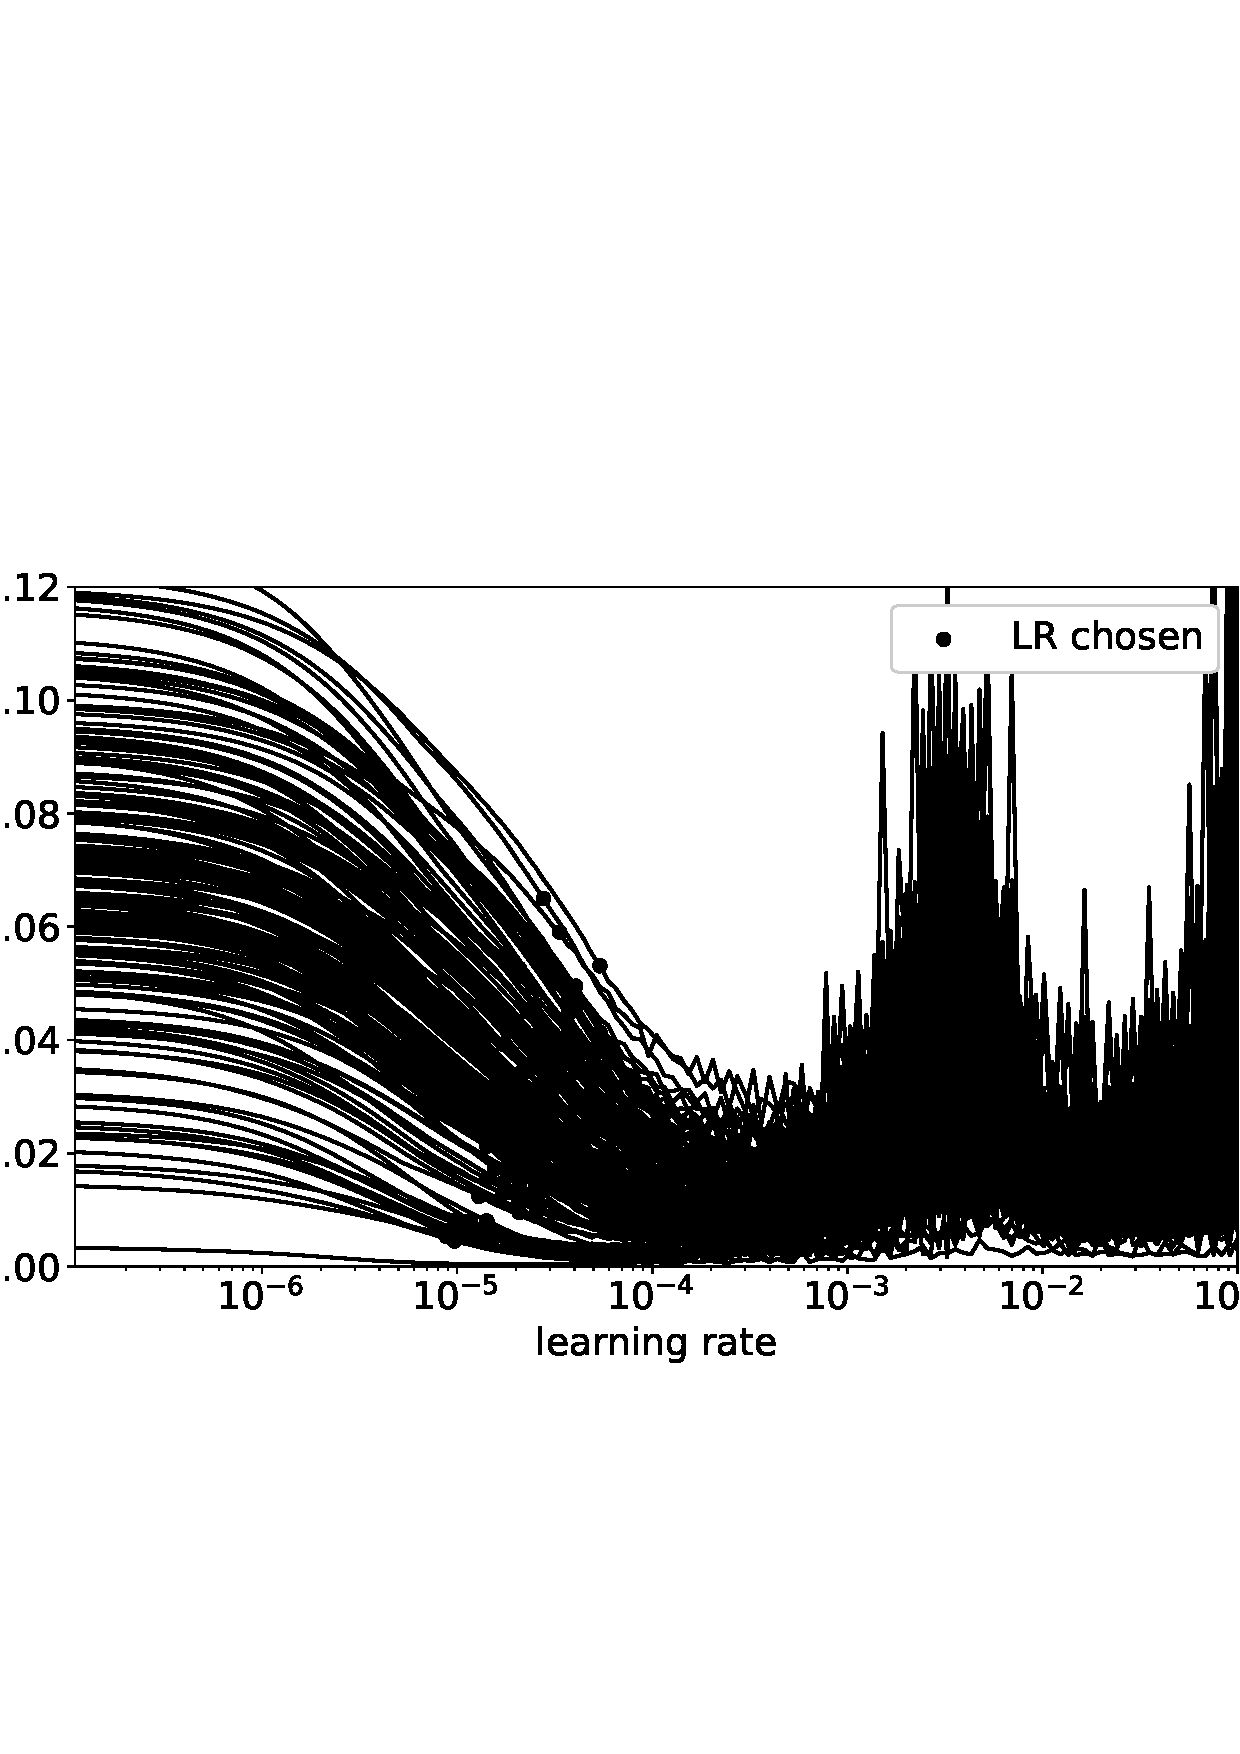
\includegraphics[width=\textwidth]{learning-rate.png}
\caption{Left: LR finder plots for a subset of images. Each line describes the inpainting loss for one iteration at different learning rates. Low LRs (left) show very small differences and high LR (right) show instability. Adequate LR are found in the region with steepest negative slope (large loss reduction per iteration).  } \label{fig2}
\end{figure}

\subsection{cycleGAN}

\begin{figure}
\includegraphics[width=\textwidth]{cycleGAN-nodule-generator.png}
\caption{Nodules generation using cycleGAN. Five training examples of nodule generation using cycleGAN are shown. For each row, the image on the right is the original image with one nodule depicted inside an orange rectangle. The image on the left is the inpainted version of the image on the right. We can observe that the nodule is not visible. The images in the middle, represent, from left to right the nodule growth across various epochs using one generator from cycleGAN.} \label{fig3}
\end{figure}

\section{Discussion}
There are several points that can be improved in order to obtain a better inpainting performance qualitatively and in terms of MSE. Firstly, inpainting should be performed in a 3D fashion using 3D CNNs and using the complete information from the regions inside the lungs. The current 2D approach limits the lung information to the information in one slice. Inpainting with a 3D volume would allow the network to identify if a nodule is in contact with a vessel (XX?) .We performed preliminary experiments with this technique, but memory and execution time constrains prevented us from completing the experiments with this model.

%
% ---- Bibliography ----
%
% BibTeX users should specify bibliography style 'splncs04'.
% References will then be sorted and formatted in the correct style.
%
% \bibliographystyle{splncs04}
% \bibliography{mybibliography}
%
\begin{thebibliography}{bibliography}
\bibitem{ref_article1}
Author, F.: Article title. Journal \textbf{2}(5), 99--110 (2016)

\bibitem{ref_lncs1}
Author, F., Author, S.: Title of a proceedings paper. In: Editor,
F., Editor, S. (eds.) CONFERENCE 2016, LNCS, vol. 9999, pp. 1--13.
Springer, Heidelberg (2016). \doi{10.10007/1234567890}

\bibitem{ref_book1}
Author, F., Author, S., Author, T.: Book title. 2nd edn. Publisher,
Location (1999)

\bibitem{ref_proc1}
Author, A.-B.: Contribution title. In: 9th International Proceedings
on Proceedings, pp. 1--2. Publisher, Location (2010)

\bibitem{ref_url1}
LNCS Homepage, \url{http://www.springer.com/lncs}. Last accessed 4
Oct 2017
\end{thebibliography}
\end{document}
